\chapter{Methodology}
\label{chap:methodology}
\begin{spacing}{1.5}
This chapter details the methodological workflow for designing and implementing the GNA QA system. The system leverages a RAG pipeline tailored to the Geoportale Nazionale per l’Archeologia (GNA) knowledge base (KB). It comprises modular components for data acquisition, preprocessing, retrieval, generation, feedback collection, and evaluation. The methodology evolved through iterative development: beginning with a prototype and advancing to a full-scale system with custom components optimised for resource efficiency. In doing so, the chapter outlines the broader methodological framework and the concrete steps undertaken, offering an in-depth account of the design choices, technical architecture, data preparation, implementation, and evaluation processes.


\section{Prototype}
The initial prototype served as a proof-of-concept, developed to validate the feasibility of applying RAG to the case study and to identify early challenges. The system integrated a minimal pipeline built with LangChain\footnote{LangChain is an open-source and Python-centric framework designed to simplify the development of applications powered by LLMs. For further details and practical examples, consult the official documentation at \url{https://python.langchain.com/docs/introduction/}.}\nocite{noauthor_langchain_2024} -- an off-the-shelf tool widely adopted for coordinating retrieval and generation tasks \citep{mishra_using_2024,akkiraju_facts_2024} -- to combine vector-based retrieval and LLM generation within an interactive environment.

\subsection{System Design}
The prototype architecture (\autoref{fig:protosys}) consisted of:
\begin{itemize}
      \item \textbf{knowledge base}: a CSV dataset created from the web-based operational manual of the Geoportale Nazionale dell’Archeologia (GNA). Content was pre-processed into document chunks enriched with metadata (titles, URLs, descriptions);
      \item \textbf{vector store}: semantic embeddings of chunks were computed using MistralAI API and then stored in a FAISS database;
      \item \textbf{generation language model}: the Mistral \textit{NeMo} LLM was accessed via the same Mistral API for answer generation;
      \item \textbf{retrieval mechanism}: queries were embedded and matched against FAISS; all retrieved chunks were concatenated into a single context and passed to the Mistral model;
      \item \textbf{user interface}: a front-end implemented via Streamlit (\autoref{fig:proto_UI}) allowed users to input queries in natural language and visualise answers in a clean, accessible format.
\end{itemize}


\begin{figure}[H]
  \centering
  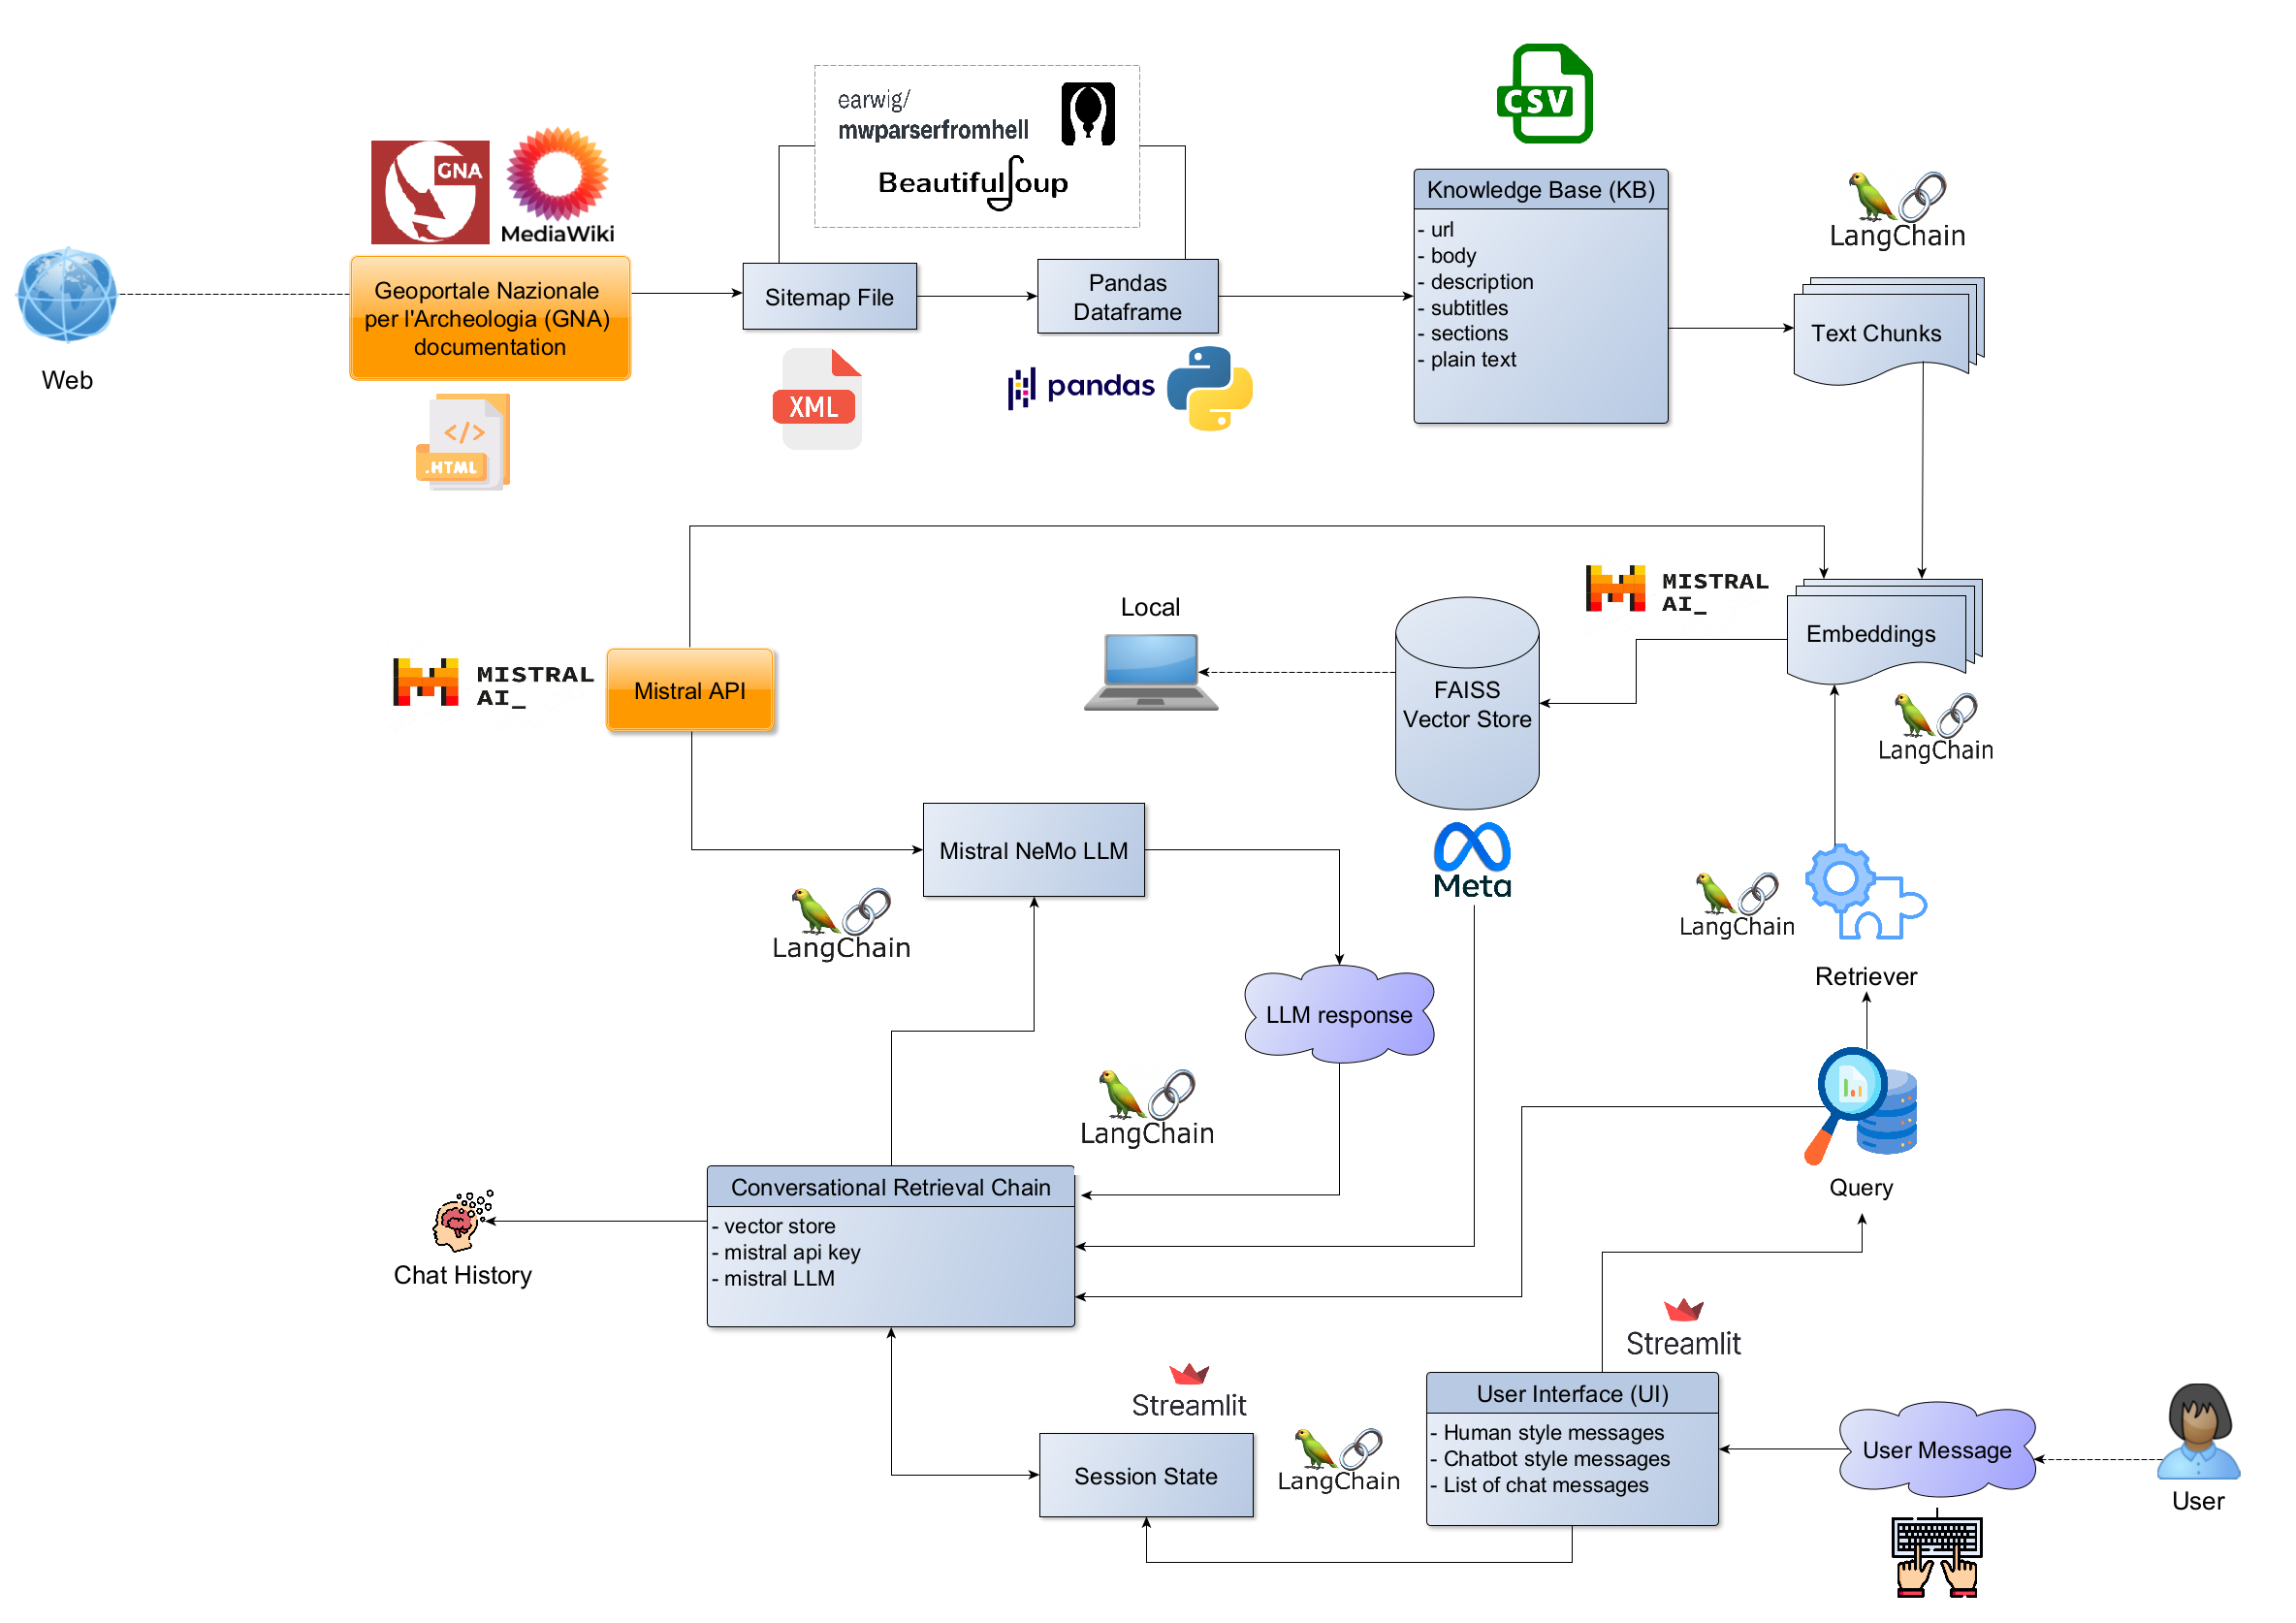
\includegraphics[width=\textwidth]{images/prototype_diagram.png} 
  \caption{Prototype system architecture.}
  \label{fig:protosys}
\end{figure}

\begin{figure}[H]
  \centering
  
\includegraphics[width=\textwidth]{images/proto_UI.png} 
  \caption{Prototype user interface deployed on Streamlit Community Cloud.}
  \label{fig:proto_UI}
\end{figure}

LangChain served as the orchestration layer, providing ready-made abstractions that connected data ingestion, retrieval, and generation into a single workflow (\autoref{fig:prototype-pipeline}). Concretely, it handled prompt templating for the Mistral \textit{NeMo} model, mediated the \texttt{Conversational Retrieval} flow, and maintained short-term dialogue state through \texttt{ConversationBufferMemory}. The retriever was based on a FAISS vector store, which indexed chunked representations of documents and returned the top-$k$ semantically similar chunks given a user query. Retrieved chunks were then combined using LangChain’s \textit{stuff} method\footnote{In LangChain, the stuff method is a particular abstraction for context packing. It concatenates the top-$k$ retrieved documents and inserts the combined block into a single prompt template passed to the LLM. While computationally lightweight, it is limited by the model’s context window. LangChain also provides alternative strategies such as \textit{map-reduce}, \textit{refine}, and \textit{map-rerank} \citep{topsakal_creating_2023}.} (\autoref{lst:stuff-method}), in which all documents are concatenated into a single prompt template and passed to the LLM.

\vspace{0.8em}
\begin{figure}[H]
\centering
\begin{adjustbox}{max width=\linewidth}
\begin{tikzpicture}[
  node distance=2.2cm,
  every node/.style={rectangle, draw, rounded corners, minimum width=2.8cm, minimum height=1cm, align=center},
  arrow/.style={-{Latex[length=3mm]}, thick}
]

\node (query) {User query};
\node (retriever) [right=of query] {Retriever \\ (FAISS)};
\node (context) [right=of retriever] {Context packing \\ (\textit{stuff} method)};
\node (generation) [right=of context] {LLM generation};

\draw[arrow] (query) -- (retriever);
\draw[arrow] (retriever) -- (context);
\draw[arrow] (context) -- (generation);

\end{tikzpicture}
\end{adjustbox}
\caption{Prototype retrieval pipeline: from user query to generation via retrieval and context packing.}
\label{fig:prototype-pipeline}
\end{figure}

The appeal, methodologically, privileged rapid deployment over optimisation, with the primary aim of validating the pipeline: a single Pythonic framework glued together embedding creation, vector search, prompt assembly, and LLM calls, enabling a minimal viable product that validated feasibility before investing efforts in bespoke infrastructure.


\begin{lstlisting}[language=Python, 
                  breaklines=true,
                  frame=none, 
                  showspaces=false,
                  showstringspaces=false,
                  showtabs=false,
                  caption={Usage example of the stuff method from LangChain.}, 
                  captionpos=b, 
                  label={lst:stuff-method},
                  xleftmargin=0.05\textwidth,
                  xrightmargin=0\textwidth]
from mistralai import Mistral
from langchain_mistralai import ChatMistralAI
from langchain.memory import ConversationBufferMemory
from langchain.chains import ConversationalRetrievalChain
from langchain.prompts import (
    ChatPromptTemplate,
    HumanMessagePromptTemplate,
    SystemMessagePromptTemplate,
)

def get_conversation_chain(vector_store, api_key: str, model_name: str, system_message:str, human_message:str):
    """
    Create a conversational retrieval chain with a Mistral LLM.

    The chain uses LangChain's ConversationalRetrievalChain with the 
    default "stuff" document combination strategy, concatenating the 
    retrieved chunks into a prompt template. A ConversationBufferMemory 
    maintains chat history across turns, enabling stateful interaction.

      Args:
        vector_store: The vector database wrapper (FAISS) used for retrieval.
        api_key (str): API key for the Mistral LLM.
        model_name (str): Identifier of the Mistral model to be used.
        system_message (str): The system-level instruction in the prompt.
        human_message (str): The user-facing prompt template.

      Returns:
        conversation_chain: A ConversationalRetrievalChain instance ready 
        for query-answering with memory support.
      """

    llm = create_mistral_llm(api_key, model_name)
    
    # Configure memory for conversation history
    memory = ConversationBufferMemory(memory_key="chat_history", return_messages=True)

    conversation_chain = ConversationalRetrievalChain.from_llm(
        llm=llm,
        retriever=vector_store.as_retriever(),
        memory=memory,
        rephrase_question=False,
        combine_docs_chain_kwargs={
            "prompt": ChatPromptTemplate.from_messages(
                [
                    system_message,
                    human_message,
                ]
            ),
        },
    )
    return conversation_chain
\end{lstlisting}



At the same time, the prototyping phase exposed several framework frictions that informed the later redesign. One issue concerned redundant model calls within the LangChain stack -- most notably the automatic query rephrasing in \texttt{ConversationalRetrievalChain} -- which doubled LLM invocations and increased the risk of hitting API rate limits. This was mitigated through a simple rate-limiting guard with a one-second delay, but the solution remained suboptimal. A second problem arose with the retry logic in \texttt{MistralAIEmbeddings}, which failed to handle \texttt{HTTP 429} \textit{Too Many Requests}\footnote{The HTTP 429 \textit{Too Many Requests} status code signals that the client has exceeded the allowable number of requests within a specified timeframe. This response enforces what is commonly known as \textit{rate limiting}, instructing the client to reduce its request frequency.} responses correctly due to a bug in LangChain’s client error handling. This reduced robustness under bursty traffic until an upstream patch was introduced later on,\footnote{Pull request addressing the incorrect exception handling for rate limiting in \texttt{MistralAIEmbeddings} emerged in LangChain \href{https://web.archive.org/web/20250823161804/https://github.com/langchain-ai/langchain/pull/29242}{PR\#29242} and it was released in the subsequent version (January 2025).}\nocite{noauthor_mistralai_2025} but the episode highlighted the limited control over low-level failure modes. Finally, reliance on predefined chains restricted experimentability by limiting chunk-level metadata control and constraining the ability to vary context-packing strategies or introduce custom pre- and post-processing filters without abandoning the abstraction layer altogether.

These findings, which emerged during implementation and debugging, motivated a shift toward a more modular pipeline. In this redesign, chunking, vectorisation, and retrieval, were configured and evaluated explicitly, avoiding reliance on predefined chains and granting finer control over performance-critical components.

\subsection{Evaluation}
The evaluation of the system's prototype followed a pronged path:
\begin{enumerate}
      \item \textbf{Human assessment}: responses were manually annotated on a 5-point Likert scale for consistency, fluency, completeness, and relevance, following best practices in human-centred evaluation of dialogue systems \citep{abeysinghe_challenges_2024,van_der_lee_human_2021};
      \item \textbf{LLM-as-a-judge}: an external model -- namely, OpenAI’s GPT-3.5 -- was prompted in a few-shot setting to automatically score responses across the same criteria, producing an additional layer of intrinsic evaluation \citep{svikhnushina_approximating_2023}.
\end{enumerate}

This custom approach reflected the broader methodological challenges in evaluating RAG systems, where traditional automatic metrics -- e.g., BLEU, ROUGE, METEOR, etc. -- have shown limited reliability in dialogue contexts (cf. \autoref{sec:eval_and_bench}).

\subsection{Insights for System Redesign}
Prototyping revealed several challenges that guided the design of the subsequent system:
\begin{itemize}
      \item \textbf{Scalability:} reliance on CSV storage and naive concatenation of retrieved chunks limited efficiency and made the system unsuitable for larger-scale deployments.
      \item \textbf{Resource efficiency:} redundant LLM calls (e.g., for query rephrasing in LangChain) caused unnecessary latency and risked exceeding API rate limits.
      \item \textbf{Metadata control:} the absence of fine-grained chunk-level metadata management constrained retrieval flexibility.
      \item \textbf{Evaluation scope:} intrinsic evaluation without a gold standard or baseline system restricted comparability with other solutions; user and domain-expert feedback was absent at this stage.
      \item \textbf{Dependency on third-party frameworks:} reliance on LangChain introduced constraints in terms of customization and debugging transparency, limiting the control over specific components.
      \item \textbf{Limited multilingual support:} initial prototype focused primarily on Italian, with limited capabilities for handling cross-lingual queries or documents.
      \item \textbf{Simplistic retrieval:} the use of basic dense retrieval without exploring hybrid or advanced reranking techniques may have constrained retrieval effectiveness.
      \item \textbf{Lack of user feedback integration:} the prototype did not incorporate mechanisms for collecting and utilising user feedback to iteratively improve system performance.
      \item \textbf{Narrow evaluation metrics:} assessment relied mainly on subjective human ratings and LLM-based scoring, without the inclusion of broader quantitative measures.
      \item \textbf{Absence of real-world testing:} the prototype was not deployed in a live environment, preventing the observation of actual user interaction patterns and limiting insights into robustness under realistic conditions.
\end{itemize}

These limitations underscored the need for a more scalable and systematically evaluated architecture, motivating the full system design presented in \autoref{sec:full_system}. In parallel, the prototype confirmed the viability of the RAG approach, offering crucial insights into system bottlenecks that directly informed the subsequent design choices.


\section{Full-Scale Implementation}\label{sec:full_system}
The full system was re-engineered from scratch to support dynamic, scalable document ingestion, contextual retrieval, and answer generation using open-source language models. All LangChain dependencies were removed in favour of custom Python implementations to improve modularity, debugging transparency, and flexibility in processing. The final architecture (fig. xx) includes:
\begin{itemize}
      \item a custom KB construction module, which integrates sitemap generation and web-crawling,
      \item semantic chunking and metadata enrichment,
      \item MistralAI-based vector embeddings,
      \item a FAISS vector store for retrieval,
      \item a generation module with open-source Mistral \textit{NeMo} model,
      \item generative responses with inline citation handling,
      \item a reactive front-end Streamlit interface,
      \item and a feedback management system.
\end{itemize}

Together, these modules amount to a complete end-to-end system. Web documents are ingested, cleaned, and segmented; semantic metadata and embeddings are created; retrieval is performed over a dedicated vector store; and answers are generated, presented through an interactive interface, and enriched by user feedback mechanisms. The outcome is not a loose set of tools, but a coherent workflow that moves seamlessly from source material to user-facing response, capable of supporting real use in the GNA context.

\sloppy
\section{Data Acquisition and Preprocessing}
\subsection{Sitemap Generation}
The sitemap is constructed via a focused breadth-first crawler targeting the MediaWiki documentation -- accessible at \url{https://gna.cultura.gov.it/wiki} -- which hosts the official user manual of the GNA \citep{mic_mic_2019}. 

The crawler is configured to:
\begin{itemize}
      \item begin at the root node (\texttt{\href{https://web.archive.org/web/20250803092155/https://gna.cultura.gov.it/wiki/index.php/Pagina_principale}{Pagina\_principale}}\nocite{noauthor_wiki_2025});
      \item follow only internal links matching \texttt{/wiki/index.php/}, excluding irrelevant namespaces such as \texttt{Special:}, \texttt{User:}, or \texttt{Talk:};
      \item normalise URLs by removing query parameters to prevent duplicates;
      \item apply a polite crawling policy, including a one-second delay between requests and a custom user-agent header;
      \item limit traversal with a maximum crawl depth\footnote{Crawl depth is intended as the maximum number of link ``level'' away from the starting url that the crawler will follow.} of 10 and page limit\footnote{Page limit parameter refers to the maximum number of pages the crawler will visit and include in the sitemap, regardless of depth.} set to 200 pages.
\end{itemize}

The output is a structured sitemap serialised as an XML file (\texttt{GNA\_\_sitemap.xml}), annotated with metadata such as last-modified timestamps, priority, and update frequency. This sitemap then provides the foundation for all subsequent document harvesting and processing steps.

\subsection{Document Crawling}
The next stage systematically collects the contents of all URLs listed in the sitemap to ensure comprehensive coverage of the manual. Pages are fetched asynchronously with retry logic, exponential backoff, and controlled concurrency to withstand transient network issues or throttling. Requests are interleaved with pauses to avoid overwhelming the server and failed URLs are logged for reprocessing.

Once retrieved, the raw HTML is parsed using BeautifulSoup, focusing on the main content (\texttt{deiv\#mw-content-text}) and stripped of extraneous elements such as navigation bars, footers, and other layout components that do not contribute semantic content. The remaining material is processed preserving the logical reading order. Structural features are carefully retained: section headers (\texttt{h1-h6}) are used to reconstruct a hierarchical outline of the page; paragraphs, tables, lists, and images are preserved as discrete items, each linked back to its contextual breadcrumb trail. This ensures that the captured content is situated within its original navigational hierarchy, which later supports more precise retrieval.

The outcome of this step is a collection of structured representations of the user manual’s pages, where meaningful content is disentangled from noise and the logical organisation of the source is preserved.


\subsection{Chunking}
After parsing, documents are segmented into smaller and more manageable units. To this end, the system employs a sliding-window strategy with a maximum span of 512 characters and an overlap of 128, a configuration recommended to favour dense retrieval while mitigating excessive fragmentation of context \citep{wang_searching_2024}.

Chunks are not treated as inert slices of text, but as semantically enriched units that carry a set of contextual signals. Each one is assigned a unique identifier -- a SHA-256 hash of its source and position -- and is accompanied by the source URL, page title, and the chain of section headers that serve as navigational breadcrumbs. Content is further annotated with keywords extracted through the \textit{KeyBERT} method\footnote{\textit{KeyBERT} is a keyword extraction technique which uses BERT embeddings to generate the keywords and keyphrases most closely aligned with a document.} and named entities identified with the model \textit{it\_core\_news\_md} from spaCy. The metadata also records the content type -- whether a passage of text, a table, a list, or an image -- ensuring that the heterogeneous nature of the original source remains visible at retrieval time.

\textbf{Tables. }Tables are preserved as autonomous chunks formatted in Markdown, maintaining both their structure and interpretability. 

\textbf{Lists. }Lists are likewise extracted as discrete units, safeguarding their enumerative character. 

\textbf{Images. }Images are handled with particular care, since they frequently consist of illustrative diagrams, tables embedded as graphics, or screenshots of the GNA QGIS plugin (cf. \autoref{sec:gna_plugin}) that can be of value for the retrieval and answer generation stages. To unlock this layer of information, the system applies an OCR pipeline built on Tesseract, enhanced with a series of pre-processing steps. Each image is first converted to greyscale and rescaled through bicubic interpolation to sharpen textual contours, then contrast-limited adaptive histogram equalisation (CLAHE) is applied to reduce noise and improve legibility across varied backgrounds. The processed image is passed to Tesseract with a configuration optimised for Italian language recognition and extended character support, allowing the extraction of structured textual surrogates. These OCR outputs are integrated into the retrieval space as additional content, making usable otherwise inaccessible visual information.

The overarching principle guiding this design is that chunking must adapt to the structure of the document rather than obey a rigid, uniform rule (cf. \autoref{fig:chunking_approach}). Accordingly, the approach combines sentence-based splitting for textual passages -- ensuring units remain compact and well-suited for dense retrieval -- with boundary-based segmentation for structural elements such as tables, lists, and images, which act as natural delimiters. This custom strategy avoids the weaknesses of relying exclusively on one paradigm: purely sentence-driven methods risk breaking semantic continuity, while purely boundary-driven approaches tend to produce uneven or oversized segments (\textcolor{blue}{Microsoft Learn,} \citeyear{noauthor_develop_2025}).

\vspace{0.8em}
\begin{figure}[H]
  \centering
  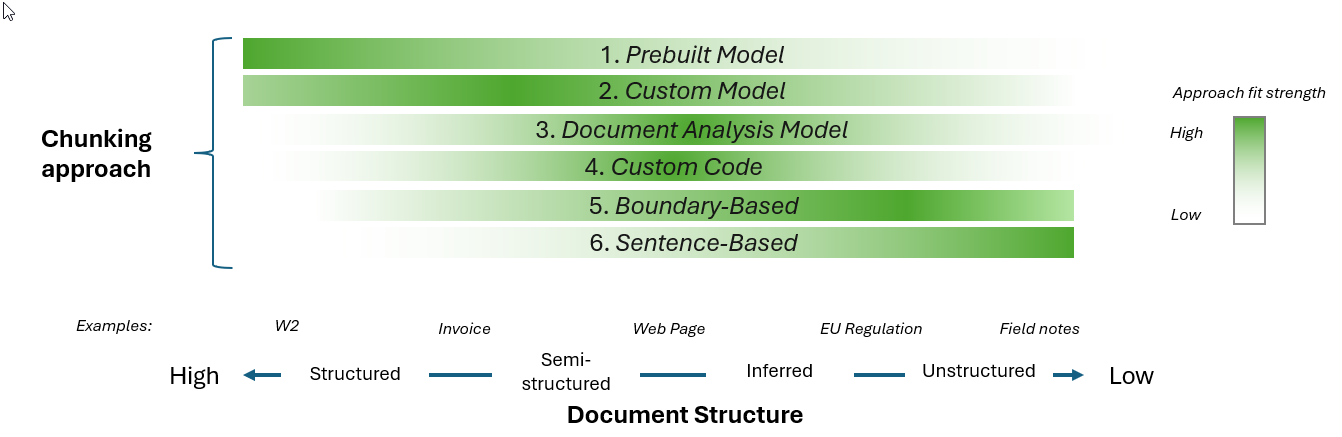
\includegraphics[width=\textwidth]{images/chunking-approaches-by-document-structure.png} 
  \caption{Different chunking strategies according to document structure.\\
  \footnotesize{Source: \href{https://web.archive.org/web/20250825093743/https://learn.microsoft.com/en-us/azure/architecture/ai-ml/guide/rag/rag-chunking-phase}{Microsot Learn}}.}
  \label{fig:chunking_approach}
\end{figure}

Such tailoring proves especially important in the archaeological domain, where textual exposition often coexists with structured metadata, tabular references, and visual documentation. The resulting knowledge base is one that strikes a careful balance: granular enough to be tractable for retrieval, yet faithful enough to preserve the integrity of the original material. In practice, this balance enhances retrieval precision and ensures that the content of the GNA user manual -- complex, layered, and semi-structured -- remains interpretable in downstream processings.

Finally, all enriched chunks are serialised into a JSON file,\footnote{Output: 835 structured chunks saved in \texttt{data/chunks\_memory.json}.} which constitutes the data source for embedding, retrieval, and generation tasks. This modular format ensures transparency and traceability of the preprocessing pipeline and enables flexibility to experiment with alternative retrievers, query rewriting techniques, and reranking strategies as outlined in \autoref{sec:exp_ablation}.

\sloppy
\subsection{Vector Embeddings}
Document chunks are converted into dense vector representations using the \textit{intfloat\/multilingual-e5-large} model from Sentence Transformers. This model was selected for its multilingual encoding capabilities and strong performance in semantic retrieval tasks, making it suitable for the predominantly Italian KB while allowing also cross-lingual queries. 

Text chunks are processed in batches and transformed into L2-normalised embeddings to ensure vector magnitudes are uniform. Embeddings are cached locally to avoid redundant computation across runs. The normalised vectors are stored in a FAISS \texttt{IndexFlatIP} index, which performs brute-force nearest neighbor search using the inner product (dot product) as metric. Alongside the vector index, a separate metadata store is maintained, linking each embedding to its corresponding chunk through a unique identifier. This separation enables efficient similarity search in FAISS while preserving quick access to rich metadata such as source URL, document structure, and content type for downstream processing.\footnote{Output: FAISS index stored in \texttt{.faiss\_db}, linked with its metadata.}

These embeddings and their associated metadata form the foundation for the retrieval stage, where user queries -- also encoded with the same \textit{multilingual-e5-large} model, to guarantee that both queries and documents share the same normalised vector space -- are matched against the stored vectors to identify the most semantically relevant chunks for answer generation.

\section{Candidates Retrieval}
When a user submits a query, it is embedded using the same encoder to ensure vector space consistency. The FAISS index, configured for inner-product similarity, is queried to return the top-$k$ candidate chunks.\footnote{The default value of \texttt{k=5} was determined empirically to balance response quality and token constraints.} Retrieval is executed entirely within the vector space to maximise speed and maintain consistent scoring across CPU-based deployments. The retrieved results are enriched with their stored metadata, which includes source URL, document title from the original web section, hierarchical section headings, and content type (text, table, image). Candidates are then grouped by provenance, ensuring that related chunks from the same source URL are passed together into the generation stage, thus improving contextual coherence, supporting inline citation, and reducing redundancy.

To further improve factual density, a lightweight filtering heuristic is applied to penalise very short or contextless chunks, deprioritising fragments that lack substantive information. The grouped and filtered candidates are returned as structured context objects, ready to be consumed by the answer generation module. 

This retrieval framework serves as the baseline for subsequent ablation studies described in the evaluation phase (cf. \autoref{sec:exp_ablation}), where alternative retrieval strategies and scoring variations are tested against this reference implementation.

\subsection{Experimental Setup for Ablation Studies}\label{sec:exp_ablation}
To systematically evaluate the contribution of different retrieval strategies. we conducted a series of ablation experiments. In this context, \textit{ablation} refers to the systematic removal, isolation, or modification of system components in order to evaluate their specific effect on overall performance. Importantly, none of the tested approaches was permanently integrated into the main pipeline; instead, each configuration was evaluated independently to allow for a broader performance comparison, as detailed in \autoref{sec:evaluation_protocol}. The results were then compared to the baseline retrieval outcomes.

The following retrieval configurations were implemented and evaluated:
\begin{itemize}
    \item \textbf{Dense retrieval.}\\
    This method employs dense vector embeddings for document representation and similarity search. It relies on FAISS as the underlying vector database, wrapped via the \texttt{VectorDatabaseWrapper} module. Queries are encoded into embeddings and compared with pre-computed document embeddings, returning the top-$k$ results ranked by inner-product similarity. Query embeddings are cached using a normalised MD5 hash to avoid redundant computations, and batch querying is supported.
    \item \textbf{BM25 retrieval.}\\ 
    A traditional sparse retriever based on the BM25 algorithm. The index was constructed over concatenated metadata fields -- \texttt{title}, \texttt{keywords}, \texttt{headers\_context}, and \texttt{document} -- from the same chunks metadata store. Preprocessing was applied specifically for Italian, including stopword removal, stemming, and handling of clitics and apocope forms. The tokenised corpus was then indexed for lexical matching. As with dense retrieval, a batch mode was implemented. The default cutoff parameter (k = 5) was selected empirically to balance response quality against tokenisation and latency constraints.
    \item \textbf{Hybrid retrieval.}\\ 
    To combine semantic similarity with lexical matching, hybrid retrieval strategies were explored. Two fusion techniques were implemented:
    \begin{itemize}
            \item \textbf{Weighted Reciprocal Rank Fusion (RRF):} ranks from dense and sparse retrievers are aggregated using RRF. The fusion score for document $d$ is computed as:
\[
\frac{w_\mathrm{dense}}{k + \mathrm{rank}_\mathrm{dense}} + \frac{w_\mathrm{sparse}}{k + \mathrm{rank}_\mathrm{sparse}} ;
\]
where the default weights parameters were $w_{\text{dense}} = w_{\text{sparse}} = 1.0$, candidates set size = 50, and \text{\texttt{k}} = 60.
            \item \textbf{Score-blend fusion:} here, normalised scores from the two retrievers are merged using a custom blending function that allows for fine-tuning the influence of each method:
\[
S_{\text{norm},d} = \frac{S_d - \min(S_d)}{\max(S_d) - \min(S_d)}, \quad  
S_{\text{norm},s} = \frac{S_s - \min(S_s)}{\max(S_s) - \min(S_s)} 
;\]
\[
S_h = S_{\text{norm},d} + \alpha \cdot S_{\text{norm},s} ;
\]
where $S_{\text{norm},d}$ and $S_{\text{norm},s}$ are the min-max normalised scores of the dense and sparse retrievers, respectively, and $\alpha$ controls the relative weight of the sparse component ($w_d = w_s = 1$, $k = 60$) \citep{wang_searching_2024}. Unlike RRF, this approach requires that scores from different retrievers are defined on comparable scales.
\end{itemize}
\end{itemize}
%\noindent\subsection*{\textit{\Large What to pick?}}
\vspace{1em}
\noindent{\textit{\Large What to pick?}}

The choice between RRF and Score-blend depends on the specific retrieval context. RRF is particularly suitable when score scales between retrievers are incompatible or unstable, as its rank-based aggregation is less sensitive to scale differences and prioritises consensus across retrieval methods. Conversely, Score-blend is more appropriate when per-query scores are reliable, as it allows finer control over the relative influence of dense and sparse components. Edge-case behaviours include: 
\begin{enumerate}[(a)] 
\item \textit{Document appears in only one list}: RRF ranks it lower, while Score-blend assigns it a normalised score from the contributing retriever;
\item \textit{All scores equal in a list}: Score-blend reduces the contribution of that retriever, whereas RRF still differentiates documents by rank.
\end{enumerate}


\noindent \subsubsection*{\Large Query Rewrite}
To sharpen retrieval quality, we experimented with \textit{query rewriting}, i.e. reformulating user queries to increase the likelihood of retrieving relevant documents. Within these experiments, query rewriting was conceived as a multi-strategy process that generates alternative query variants through complementary transformations, each targeting different aspects of query understanding and manipulation \citep{li_dmqr-rag_2024}. Specifically, the approach integrates:
\begin{itemize}
      \item \textbf{Core Content Extraction (CCE):} a sequence-to-sequence transformation using the \textit{it5-small} model, that rewrites the query to capture its essential informational content while removing peripheral terms.
      \item \textbf{Keyword Expansion (QE):} extraction of key terms with KeyBERT, followed by enrichment through n-gram combinations and synonym substitutions to introduce semantically related expressions.
      \item \textbf{General Query Rewriting (GQR):} linguistic normalisation based on spaCy lemmatisation and stop word removal, yielding canonical query forms.
      \item \textbf{Pseudo-Relevance Feedback (PRF):} top-ranked documents from an initial retrieval pass are analysed to extract additional high-frequency terms not present in the original query, which are then appended to the original query to form an expanded version.
      \item \textbf{Query Decomposition:} conjunctive or disjunctive queries are split into simpler sub-queries, each addressing a distinct semantic aspect.
\end{itemize}

These strategies can be applied individually or in combination (\texttt{strategy="all"}), producing a set of reformulated queries submitted to the base retriever (Dense, BM25, or Hybrid).\\


\noindent\subsubsection*{\Large Reranking}

Finally, a \textit{reranking} stage was introduced to refine retrieval outcomes.\footnote{Reranking is a post-retrieval process that reorders an initial set of candidate documents based on a more precise estimation of their relevance.} In our implementation, it operates as a wrapper around a base retriever (Dense, BM25, or Hybrid) and uses a transformer-based cross-encoder model (\textit{cross-encoder/ms-marco-MiniLM-L-6-v2}) to jointly encode the query and each candidate document, assigning a contextual relevance score. Unlike the base retriever, which typically evaluates query-document similarity using independent embeddings or lexical term matching, the cross-encoder considers full cross-attention between query and document tokens, thereby capturing finer semantic relationships.

At runtime, the reranker receives the top-$N$ candidates (with $N$ = 50) from the base retriever, tokenises each query-document pair, and performs inference in batches with mixed-precision support when available. The final output consists of a top-$k$ ranked list reordered by cross-encoder scores. This stage provided a more precise estimation of relevance, compensating for weaknesses in both dense and sparse retrieval alone.


\section{Generation}\label{sec:rag_generation}
The generation phase employs Mistral \textit{NeMo},\footnote{\url{https://web.archive.org/web/20250803120348/https://mistral.ai/news/mistral-nemo}.\nocite{noauthor_mistral_2025}} an open-source LLM accessible via a dedicated API and hosted independently. Its selection was guided by a convergence of methodological and practical requirements. First, open-source availability and a permissive licence ensured transparency, reproducibility, and the possibility of adaptation without the restrictions of proprietary services. Second, the model’s strong performance on multilingual benchmarks, including robust handling of Italian, made it particularly suitable for a system intended to operate in a cultural heritage setting where linguistic specificity is paramount. Third, Mistral \textit{NeMo} demonstrated competitive efficiency, with low latency and high throughput even when deployed on modest hardware, a quality that enabled real-time responsiveness without requiring more powerful computing infrastructures. In addition, the availability of an official API greatly facilitated seamless integration into the retrieval-augmented generation pipeline, while its ability to support extended context windows -- up to 128k tokens -- allowed the system to process multiple retrieved passages in a single prompt without truncation or loss of coherence.

While different open-source alternatives were considered too -- such as \textit{LLaMA 3}, \textit{Falcon}, \textit{Google Gemma} and \textit{OpenAI} models --, none aligned as closely with the system’s combined requirements. \textit{LLaMA 3}, for instance, offers state-of-the-art performance and strong community support, but its licensing terms restrict certain deployment scenarios and its context window is more limited in practice. \textit{Falcon} models, though efficient, have shown more variability in multilingual performance, particularly outside English. Proprietary APIs, while powerful, introduce cost barriers and potential vendor lock-in, compromising the long-term reproducibility of the research workflow. By contrast, Mistral \textit{NeMo} offered a balanced compromise: multilingual coverage, scalable deployment options, and infrastructure for fine-tuning embeddings, made it a natural fit for both the prototyping stage and the full-scale system.\footnote{For an overview between open-source and proprietary models, read \textcite{noauthor_open_2025}.}


The generation module itself is designed to deliver fluent, context-aware answers with inline citations, ensuring that responses remain both interpretable and verifiable. Prompts are constructed through a structured template combining system-level instructions (see \autoref{sec:prompt_engineering}), the user query, top-k retrieved grouped chunks, and the conversational history maintained in memory to sustain continuity across follow-ups. API calls are issued with a combination of decoding parameters: a temperature of 0.3\footnote{The parameter temperature set to 0.3 sharpens the model’s probability distribution, favouring high-likelihood tokens and suppressing unlikely alternatives, thereby producing more deterministic and factual outputs.} to prioritise factual accuracy, a top-$p$ of 0.9\footnote{The parameter top-$p$, also called \textit{nucleus sampling}, restricts generation to the smallest set of candidate tokens whose combined probability mass reaches a chosen threshold (here 90\%), ensuring that the model considers diverse but still plausible continuations while discarding unlikely options.} to maintain lexical diversity without drifting off-topic, and a maximum of 512 tokens to keep answers concise. Finally, responses undergo lightweight post-processing to enforce inline citation formatting, guarantee Italian output, and preserve readability through numbered references and paragraph boundaries.


\subsection{Prompt Engineering Techniques} \label{sec:prompt_engineering}
The system uses structured prompt engineering to ensure accurate, traceable, and contextually coherent answers. The prompt template is dynamically generated with the following components:

\noindent\subsubsection*{\large System Instructions, Boundaries and Constraints}
A custom system message (\autoref{lst:system_prompt}) is injected at the top of the prompt to guide the model’s behaviour. This message instructs the system to enforce neutrality in its answers, prioritise relevant and verifiable information, and include inline citations that correspond to metadata entries. It also explicitly discourages hallucinations and speculative responses.

\vspace{0.6em}
\begin{lstlisting}[breaklines=true,
                  frame=none,
                   caption={System prompt specifying assistant constraints and response instructions.},
                   captionpos=b,
                   label={lst:system_prompt},
  xleftmargin=0.05\textwidth,
  xrightmargin=0.05\textwidth]
system_content = """
    Sei un assistente virtuale incaricato di rispondere a domande sul manuale operativo del Geoportale Nazionale per l'Archeologia (GNA), gestito dall'Istituto Centrale per il Catalogo e la Documentazione (ICCD).

    Segui sempre queste regole:
    1. Non rispondere a una domanda con un'altra domanda.
    2. Rispondi **sempre** in italiano, indipendentemente dalla lingua della domanda, a meno che l'utente non richieda esplicitamente un'altra lingua.
    3. Cita le fonti utilizzando la notazione [numero] dove:
        - Le fonti sono fornite nel contesto della domanda e sono numerate in ordine crescente;
        - Usa numeri diversi per fonti diverse;
        - Non includere mai l'URL nel corpo della risposta;
    4. Alla fine della risposta, aggiungi un elenco di riferimenti con il seguente formato, su righe separate:
        [ID] URL completo
    5. Se non hai informazioni sufficienti per rispondere, rispondi "Non ho informazioni sufficienti".

    Le tue risposte devono essere sempre:
    - Disponibili, professionali e naturali
    - Grammaticalmente corrette e coerenti
    - Espresse con frasi semplici, evitando formulazioni complesse o frammentate
    - Complete e chiare, evitando di lasciare domande senza risposta
"""
\end{lstlisting}
\vspace{0.5em}


Each chunk passed to the LLM is numbered and grouped with its metadata (title, URL). When generating a response, Mistral is instructed to cite only the chunks used, ensuring traceability. Post-processing checks for unmatched citations or unreferenced metadata.


\section{Evaluation Protocol}\label{sec:evaluation_protocol}
Evaluation was conducted across two complementary dimensions: 
\begin{itemize}
      \item \textbf{Quantitative}, focusing on retrieval performance through metrics such as Recall (R@), Mean Reciprocal Rank (MRR@), Normalised Discounted Cumulative Gain (nDCG@), Average Precision (AP@), and Latency to assess retrieval performance;
      \item \textbf{Qualitative}, assessing the perceived quality and usability of responses through human feedback.
\end{itemize}

This dual perspective reflects the understanding that effective RAG-based QASs require not only accurate retrieval and generation but also operational efficiency and adaptability in real-world contexts \citep{akkiraju_facts_2024}. To support continuous refinement, the evaluation was designed as an iterative process, with quantitative results informing system optimisation and qualitative insights guiding user-centred adjustments.

All retrieval configurations (Dense, BM25, Hybrid, Query Rewriting, and Reranking variants) were evaluated under the same protocol, ensuring comparability of results across ablation studies. While this framework provided a coherent structure for assessment, its application also revealed several limitations inherent to the experimental setting and the available resources. These included:
\begin{itemize}
      \item \textbf{Absence of a gold standard:} there was no authoritative or verified set of annotated responses to serve as a benchmark of correctness.
      \item \textbf{No baseline system:} internal institutional tasks had no legacy solutions or established benchmarks for direct comparison in the archaeological domain.
      \item \textbf{Limited availability of domain experts:} during the early phases, development was conducted without input from real users or expert annotators; human feedback was integrated only at a later stage.
      \item \textbf{Limited applicability of automated generation metrics:} common algorithmic measures, although widely applied in text generation, have been shown to be ineffective for dialogue and QA evaluation \citep{deriu_survey_2020,liu_how_2016}.
\end{itemize}

These constraints mirror challenges identified in recent RAG evaluation literature, which emphasises the lack of standardised protocols and the importance of balancing intrinsic metrics with human-centred evaluation \citep{abeysinghe_challenges_2024}, as noted in \autoref{sec:eval_and_bench}. Akkiraju et al. (2024) further highlight the need to assess both accuracy and efficiency, pointing to critical control points in the RAG pipeline where trade-offs between retrieval quality and latency emerge.


\subsection{Datasets}\label{sec:datasets}
Widely used QA benchmarks such as SQuAD and Natural Questions or multi-hop datasets like HotpotQA \citep{yang_hotpotqa_2018} and 2WikiMultiHopQA \citep{ho_constructing_2020} are indispensable for advancing general-domain research but are misaligned with the objectives of this study. These datasets are predominantly built around encyclopaedic or factoid queries in English, often centred on entity recognition and short-span extraction. By contrast, the GNA QA system targets procedural, explanatory, and domain-specific questions expressed in Italian, where answers are not simple factual snippets but often involve step-by-step guidance, cross-references to interface components, or the interpretation of heterogeneous content.

Equally important, while KBs such as Wikipedia do consists of text that coexists with tables and lists, their role is largely illustrative or descriptive. In the GNA manual, instead, such structures are integral to the semantics of the documentation. Tables encode data entry examples or parameter constraints, lists enumerate workflows, and images -- often screenshots -- embody key instructional content. These formats are not ancillary but essential to the information needs of end-users, requiring reasoning that goes beyond the scope of existing benchmarks.

Evaluating on standard datasets would therefore risk producing misleadingly inflated scores that fail to capture the genuine challenges of domain-specific, multimodal documentation. Given these considerations, a custom evaluation set was constructed and sampled directly from the GNA KB. This ensured ecological validity, testing the QA system on the exact materials and information needs it is designed to serve.\\

\noindent To support systematic analysis, two synthetic evaluation sets were created:
\begin{itemize}
      \item \textbf{Single-hop dataset:} containing 508 queries designed to elicit single-document answers, each with a single gold document (cf. \autoref{lst:single-hop-example}). This dataset tested the system's ability to retrieve and generate answers based on isolated chunks of information.
      \item \textbf{Combined dataset:} containing 400 additional queries that require multi-hop reasoning, where answers are derived from multiple documents (2-4 chunks), for a total of 908 queries entries (cf. \autoref{lst:combined-set-example}). This dataset assessed the system's capacity to integrate information from various sources and generate coherent contextual responses.
\end{itemize}


\begin{lstlisting}[frame=none,
                   caption={JSON output format for single-hop dataset items.},
                   captionpos=b,
                   label={lst:single-hop-example},
  xleftmargin=0.2\textwidth,
  xrightmargin=0.2\textwidth]
{
  "question": "<Italian question>",
  "relevant_docs": ["<chunk_id>"],
  "document_content": "<chunk text>"
}
\end{lstlisting}

\vspace{0.6em}

\begin{lstlisting}[frame=none,
                   caption={JSON output format for combined dataset items, including single-hop and multi-hop questions.},
                   captionpos=b,
                   label={lst:combined-set-example},
  xleftmargin=0.05\textwidth,
  xrightmargin=0.05\textwidth]
{
  "question": "<Italian question>",
  "relevant_docs": ["<chunk_id_1>", "<chunk_id_2>", "..."],
  "document_content": ["<text_1>", "<text_2>", "..."],
  "is_multihop": false|true,
  "num_docs": 1|2|3|4
}
\end{lstlisting}
\vspace{0.6em}

Together, these custom test sets provided balanced coverage of both simple and complex retrieval scenarios. In both cases, questions were generated directly from the chunk corpus using Mistral \textit{NeMo} (cf. \autoref{sec:rag_generation}). For the single-hop dataset, each question was elicited from an individual chunk through a prompt that constrained the model to formulate queries strictly grounded in the given text, ensuring that answers could only be retrieved from the associated gold document. In contrast, the multi-hop dataset required a more demanding construction: subsets of two to four chunks were sampled at random, concatenated, and provided as input to the LLM with explicit instructions to generate questions resolvable only by combining information across all documents in the set. To avoid superficial overlaps, in this case the prompt enforced specificity and disallowed formulations answerable from a single source.


\subsection{Metrics}\label{sec:metrics}
To evaluate retrieval in a consistent and transparent manner, the system was assessed using a set of standard IR metrics, complemented by latency measurements to capture operational performance \citep{wang_searching_2024}:

\begin{itemize}
    \item R@5 (Recall at 5): proportion of relevant documents successfully retrieved within the top 5 results, reflecting coverage of the retrieval step;
    \item MRR (Mean Reciprocal Rank): average of reciprocal ranks of the first relevant document retrieved, rewarding systems that place the correct answer as early as possible;
    \item nDCG@5 (Normalised Discounted Cumulative Gain at 5): evaluates ranking quality by weighting relevant documents higher when they appear near the top of the result list;
    \item AP@5 (Average Precision at 5): computes the average of precision values at each point a relevant document is retrieved within the top 5, providing a balance of recall and precision across ranks;
    \item Latency: mean retrieval time per query (in seconds).
\end{itemize}

Each evaluation run stores a machine-readable report (JSON) capturing dataset name (single-hop / multi-hop), creation timestamp (UTC), orchestrator and model identifiers (Mistral API model name), retrieval parameters (top-$k$ and candidate-$k$), batch size, and device configuration. These artefacts ensure precise traceability of conditions across ablation experiments (cf. \autoref{sec:retrieval_ablation}).

\subsection{Qualitative Assessment}
To complement intrinsic metrics, qualitative evaluation focused on dimensions more directly linked to user experience:
\begin{itemize}
      \item \textbf{Relevance:} Whether the generated answer addressed the query meaningfully.
      \item \textbf{Fluency:} Linguistic naturalness and readability of responses.
      \item \textbf{Completeness:} Coverage of the key information needed to satisfy the query.
      \item \textbf{Usability:} Perceived usefulness of the system as an interactive tool.
\end{itemize}

Human feedback was collected using a lightweight rating approach (3-point Likert-scale scoring), later exported as structured datasets for analysis. Although limited in scale, this qualitative perspective provided insights into aspects of response quality that purely algorithmic metrics could not capture, particularly in relation to user trust and system transparency.



\section{User Interface}
The user interface (UI) was developed using Streamlit, chosen for its ability to support rapid prototyping and its native integration with Python NLP pipelines. Streamlit also offers built-in handling of asynchronous processes, making it well suited for a RAG system where retrieval and generation stages can vary in latency. Within the system, the UI serves as the primary interaction layer between users and the GNA QA service. Through a simple and accessible design (\autoref{fig:UI}), users are able to submit queries in natural language, receive answers, and inspect the underlying evidence via inline citations linked to the retrieved documents.

Beyond serving as a functional entry point to the system, the UI assumes a crucial methodological role. It provides a framework for integrating explicit user feedback, thereby enabling the collection of qualitative evaluations that complement quantitative retrieval metrics. Through the interface, users can annotate responses in terms of perceived relevance, fluency, completeness, and usability by selecting an option on a three-point Likert scale. These annotations generate valuable data that can be used to iteratively refine the system. As previously discussed, this human-centred dimension is particularly important in dialogue and QA contexts, where conventional automated metrics often fail to capture the subtleties of interaction quality. The interface therefore does more than display outputs: it functions as an evaluation instrument in its own right, supporting the triangulation of system performance across computational measures and human judgements.

\vspace{0.8em}
\begin{figure}[H]
  \centering
  
\includegraphics[width=\textwidth]{images/UI_full.png} 
  \caption{Streamlit user interface of GNA QA system.}
  \label{fig:UI}
\end{figure}

\noindent The application interface is organised into three main areas:
\begin{enumerate}
      \item \textbf{Sidebar:} contains MiC reference, institutional links to the GNA documentation, and contextual help describing the assistant’s capabilities. It also provides functional controls including a \textit{Clear chat history} button (``\textit{Cancella cronologia chat}'') to reset the Streamlit session (\texttt{st.session\_state.chat\_history}) and a ``\textit{Download Feedback}'' button for exporting user queries and system's responses.
      \item \textbf{Main interface:} provides a natural language input field for querying the assistant. It displays the chat history, including user messages, assistant responses and feedback buttons for each assistant reply (\autoref{fig:ratings}).
      \item \textbf{Session features}: 
      \begin{itemize}
            \item Chat history is limited to the most recent ten exchanges, which are stored and updated in the session state;
            \item Feedback from individual message indexes is stored as a set (\texttt{st.session\_state.feedback\_given}), allowing the system to prevent duplicate ratings and dynamically update UI.
      \end{itemize}
\end{enumerate}


\begin{figure}[H]
  \centering
  
\includegraphics[width=\textwidth]{images/ui_ratings.png} 
  \caption{Rating mechanism embedded in the user interface.}
  \label{fig:ratings}
\end{figure}


To guarantee smooth interactions and to minimise computational overhead, the system makes extensive use of \texttt{st.session\_state}, a built-in Streamlit object designed for persisting variables across user interactions. Unlike ordinary Python variables, which are re-initialised each time Streamlit re-runs a script, \texttt{st.session\_state} retains values for the duration of a session. This functionality is critical in a conversational application, as it allows chat memory to persist between turns. Both user queries and model responses are stored, so that continuity is preserved across multi-turn dialogues.\footnote{For more details on Streamlit session state management, see the official API documentation at \url{https://docs.streamlit.io/}.\nocite{noauthor_streamlit_2025}} 

Beyond the bounds of memory management, \texttt{st.session\_state} is also used to cache API outcomings, including responses generated by Mistral and their associated citation mappings. This prevents redundant API calls when users revisit or re-evaluate queries, at the advantage of efficiency and costs mitigation. In addition, the same mechanism is employed to track user feedback, linking annotations directly to the relevant conversational context.

To ensure a responsive user experience, the system integrates Python’s \texttt{asyncio} and \texttt{concurrent.futures} modules. Each call to the language model is executed within a new event loop, ensuring compatibility with Streamlit’s execution environment, while a \texttt{ThreadPoolExecutor} provides thread-safe parallel execution. This design enables non-blocking retrieval and generation: the interface remains responsive even under conditions of high latency or slow API responses, thus preserving a fluid user experience.


\section{Feedback Loop}
To support iterative improvement of the assistant and promote user engagement, the system integrates an interactive feedback module that allows users to rate each answer directly within the Streamlit interface. This design is intended to support continuous quality assessment and transparent evaluation of LLM-generated content.

\subsection{Collection}
As noted earlier, each assistant response is immediately followed by three clickable UI buttons based on a 3-point Likert scale:
\begin{itemize}
\item 1 point - Poor: the answer is incorrect, incomplete, or irrelevant.
\item 2 points - Fair: the answer is partially correct but lacks clarity or depth.
\item 3 points - Good: the answer is accurate, complete, and well-structured.
\end{itemize}

This mechanism is implemented using Streamlit’s interactive widgets. Once a rating is submitted, the system prevents duplicate feedback using an in-memory tracking set (\texttt{st.session\_state.feedback\_given}). The interface then displays a confirmation message (``\textit{Valutazione registrata}'', \autoref{fig:valutazione}), improving transparency.

\begin{figure}[H]
  \centering
  
\includegraphics[width=\textwidth]{images/val_registrata.png} 
  \caption{Confirmation message of registered user's feedback.}
  \label{fig:valutazione}
\end{figure}

\subsection{Storage and Export}
Feedback is stored locally in a SQLite database (\texttt{feedback.db}) with the schema specified in \autoref{lst:sql_schema}. Each record captures:

\begin{lstlisting}[language=SQL,
                  frame=none,
                   caption={SQL schema of the feedback database.},
                   captionpos=b,
                   label={lst:sql_schema},
  xleftmargin=0.2\textwidth,
  xrightmargin=0.1\textwidth]
CREATE TABLE feedback (
    id INTEGER PRIMARY KEY AUTOINCREMENT,
    timestamp TEXT NOT NULL,
    message_index INTEGER NOT NULL,
    question TEXT NOT NULL,
    answer TEXT NOT NULL,
    rating INTEGER NOT NULL
);
\end{lstlisting}

This structure supports reproducibility and traceability by maintaining a clear mapping between: the user's query string, the generated response, the rating score (1-3) and the associated timestamp (i.e., time of submission). All records are saved with minimal overhead, using parameterised SQL insertions and transaction-safe commits.

To ensure long-term preservation and collaborative accessibility of user feedback, the system implements a mechanism for periodic synchronization of collected feedback with a persistent repository. This setup enables version control over user interaction logs, supports iterative evaluation by external reviewers, and enables rollback and comparison across model updates.\footnote{This implementation is intended for controlled research use only. For production environments, sounder alternatives such as authenticated APIs and hardened database infrastructures are recommended to ensure data safety and compliance with privacy standards.}

From the sidebar, users can export all feedback as a \texttt{.csv} file using the \textit{``Esporta feedback''} functionality. This latter is powered by the \texttt{export\_feedbacks()} function, which queries the database and converts it to a downloadable format using Pandas. 

Feedback data can be used by researchers, developers, or project coordinators to assess the assistant's performance over time.


\section{Resources and Deployment}
The GNA QA system is deployed on Streamlit Community Cloud, a platform that allows developers to openly host interactive Python applications directly from a linked GitHub repository. The service abstracts most of the infrastructure overhead: each push to the repository automatically triggers a build and deployment, packaging dependencies specified in configuration files and exposing the application as a live web service. This solution enabled rapid iteration and made the system easily accessible to stakeholders without local installation.

However, long-running RAG pipelines are not trivial to host within such constrained environments. Indeed, early deployments surfaced memory leaks: object references from retrieval and generation modules, especially cached embeddings and session state artefacts, were not consistently released, leading to a progressive increase in memory usage during extended interactions. Identifying these leaking objects required targeted profiling, after which caching decorators and object reinitialisation strategies were introduced to reduce overhead. Although these optimisations improved stability, the underlying workload still proved too heavy for the default configuration availabilities of Streamlit Cloud.

To mitigate this, we contacted the Streamlit team directly and requested additional resources. As a result, the hosting environment was scaled up to 8 gibibytes (GiB), a critical increase that allowed the application to sustain concurrent sessions and longer conversational histories without interruption. 

This experience underlines a broader methodological point: deploying RAG systems is not merely a matter of algorithmic optimisation but also of infrastructure alignment, where careful monitoring, memory management, and resource planning or negotiation are essential to ensure reliability and usability under real-world usage conditions.

\subsection{Memory Management}
As discussed above, deploying a RAG workflow with multiple NLP resources integrated into a single pipeline poses considerable challenges for environments lacking access to GPUs or large memory allocations, such as free hosting platforms like Streamlit Community Cloud. To keep the system sustainable under these constraints, several optimisation strategies were adopted in terms of memory management:
\begin{itemize}
\item \textbf{Garbage collection routines:} explicit calls to Python's garbage collector (\texttt{gc.collect()}) were introduced to free unused memory between embedding and response generation steps;
\item \textbf{Batch processing:} document chunks are processed in batches to minimise memory overhead, especially during retrieval;
\item \textbf{Lazy loading:} all embeddings are computed once and stored persistently. At application startup, only the metadata is loaded into memory, and the FAISS index is accessed through memory-mapping to reduce RAM footprint;
\item \textbf{Asynchronous processing:} Streamlit's async capabilities are leveraged to keep the UI responsive while background tasks run in parallel, preventing memory spikes during long-running operations;
\item \textbf{Cache clearing policies:} \texttt{st.session\_state} objects are pruned after each session or upon manual reset by the user to prevent memory bloating during prolonged use.
\end{itemize}

\subsection{Computational Constraints Mitigation}
To counterbalance the limitations of operating under strict computational constraints and preserve system responsiveness, the following strategies were introduced:
\begin{itemize}
\item \textbf{Model selection:} the use of \textit{intfloat/multilingual-e5-large} for embedding provides a trade-off between semantic accuracy and compute efficiency, even without GPU acceleration;
\item \textbf{API offloading:} offloading generative tasks to the external Mistral API prevents the local system from being overloaded and allows scaling independently of front-end performance;
\item \textbf{Timeout and fallback handlers:} if the generation request exceeds 10 seconds or fails (e.g., due to API rate limits), the interface returns a graceful fallback response, allowing users to retry without crashing the app;
\item \textbf{Asynchronous I/O:} for embedding, retrieval, and response generation, asynchronous requests reduce UI freezing and ensure smoother user experience even under high latency conditions.
\end{itemize}


\section{Ethics and Data Governance}
The GNA QA system has been developed with sustained attention to ethical considerations and data governance, particularly in the context of cultural heritage and public information. Transparency is pursued through open release of the source code and documentation of the pipeline -- covering models, prompts, parameters --, together with versioned configurations, and machine-readable evaluation artefacts; per-run JSON logs record dataset IDs, model identifiers, and retrieval settings, all of which are made accessible through the project’s GitHub repository. Privacy is safeguarded by design, as the system processes no personally identifiable information and relies exclusively on publicly available or openly licensed materials. Licensing constraints are respected, as all resources -- from the knowledge base to the language models and software libraries -- are drawn from projects distributed under permissive terms that guarantee lawful reuse in research and educational contexts. Auditability is ensured through persistent logging of system performance and user feedback on Streamlit Community Cloud.

On the whole, these practices turn abstract commitments -- provenance, privacy, licensing, and auditability -- into concrete safeguards, allowing the GNA QA system to remain technically reliable and also a responsible instrument for public engagement.

\end{spacing}
